%!TEX root = ../paper.tex
%Ferdosi Sets 1
\begin{subfigure}{0.3\textwidth}
	\centering
	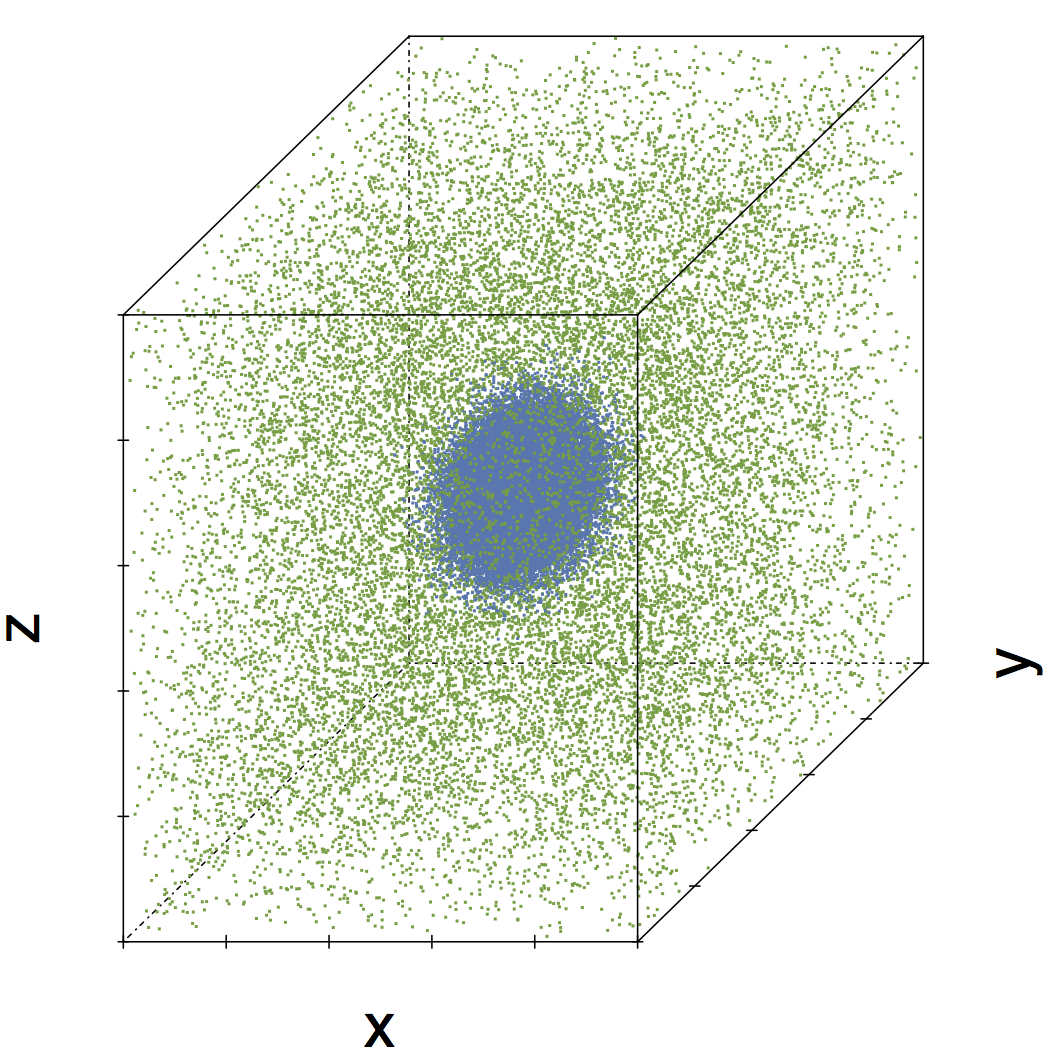
\includegraphics[width=\textwidth]{3/img/datasetplot_ferdosi_1_60000.png}
	\caption{Set \ferdosiOne}
	\label{fig:3:simulated:datasets:ferdosi1}
\end{subfigure}
% Ferdosi Set 2
\begin{subfigure}{0.3\textwidth}
	\centering
	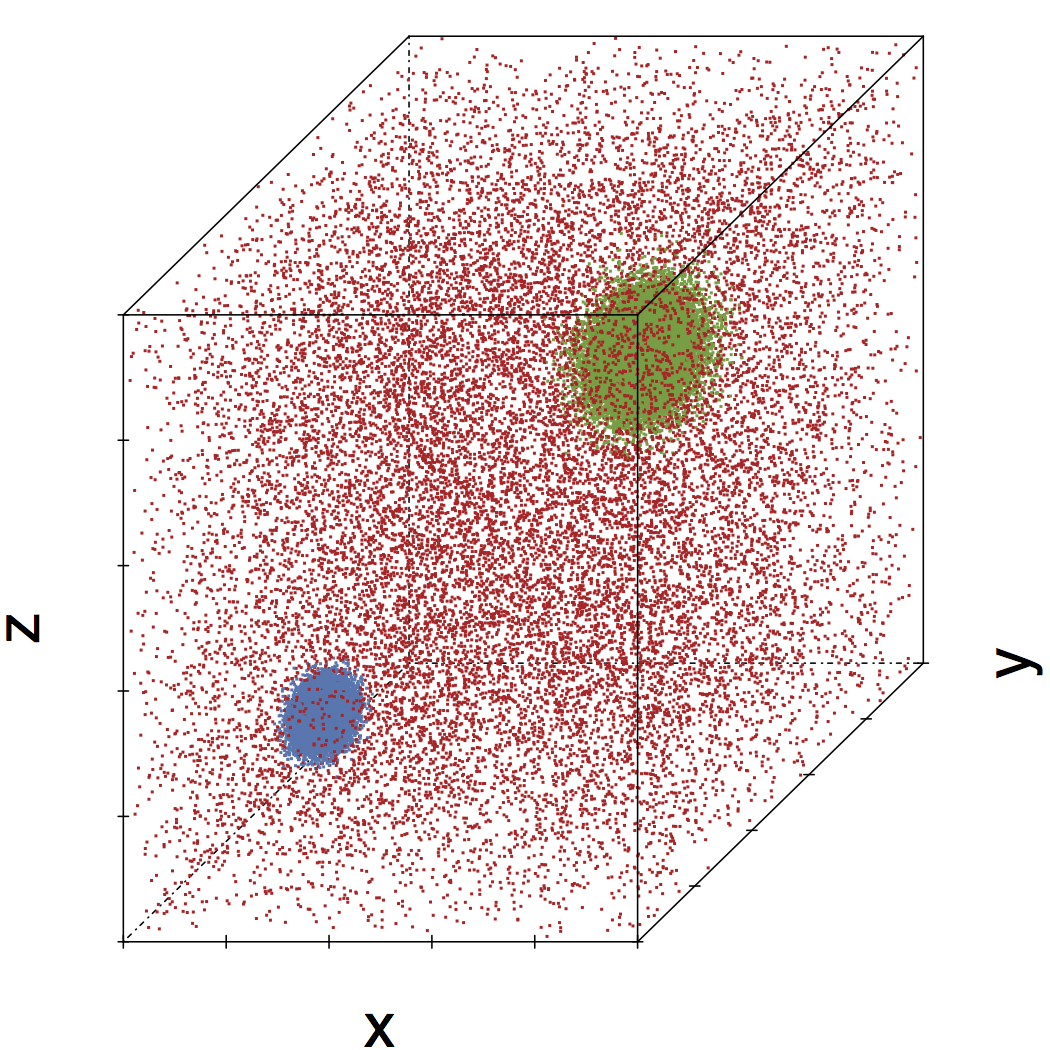
\includegraphics[width=\textwidth]{3/img/datasetplot_ferdosi_2_60000.png}
	\caption{Set \ferdosiTwo}
	\label{fig:3:simulated:datasets:ferdosi2}
\end{subfigure}	
% Ferdosi Set 3
\begin{subfigure}{0.3\textwidth}
	\centering
	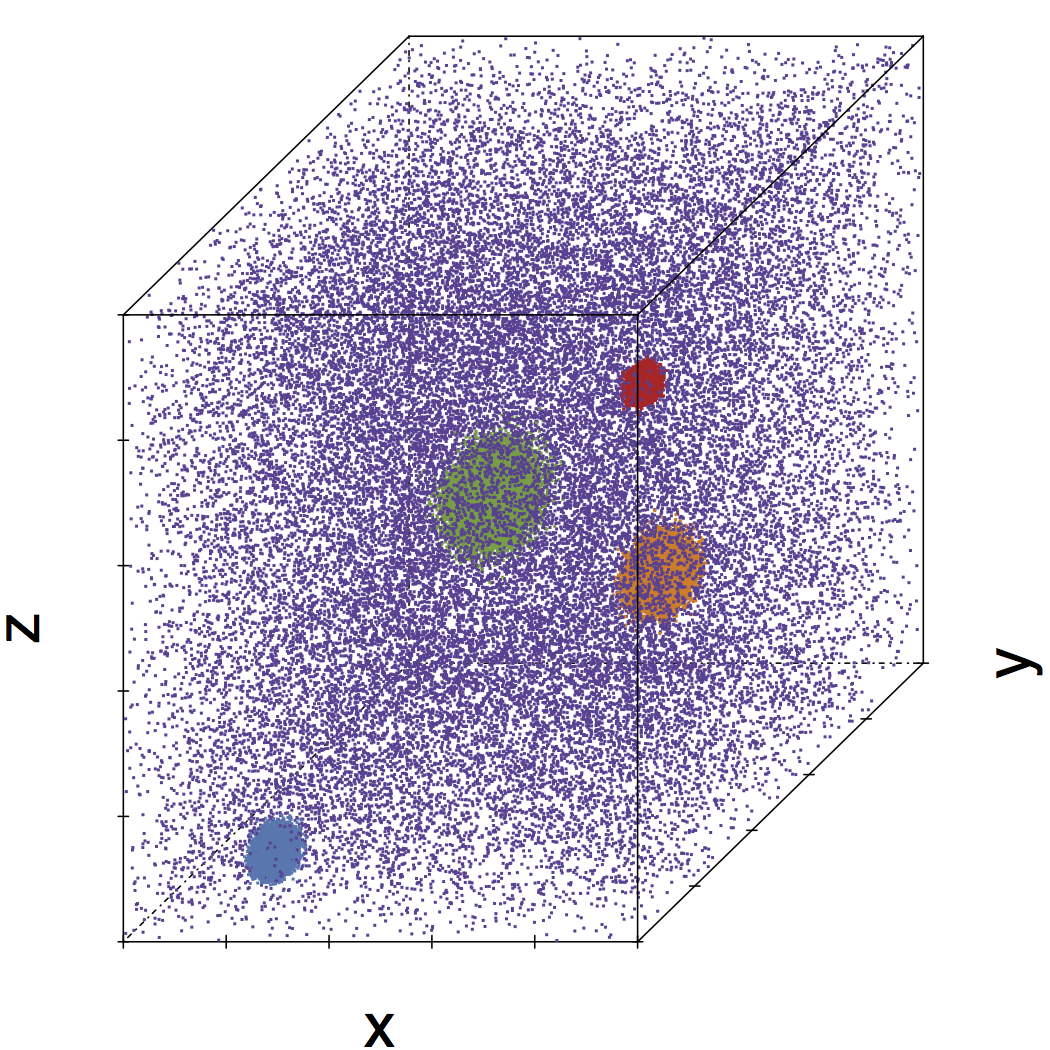
\includegraphics[width=\textwidth]{3/img/datasetplot_ferdosi_3_120000.png}
	\caption{Set \ferdosiThree}
	\label{fig:3:simulated:datasets:ferdosi3}
\end{subfigure}		
% Baakman 1	
\begin{subfigure}{0.3\textwidth}
	\centering
	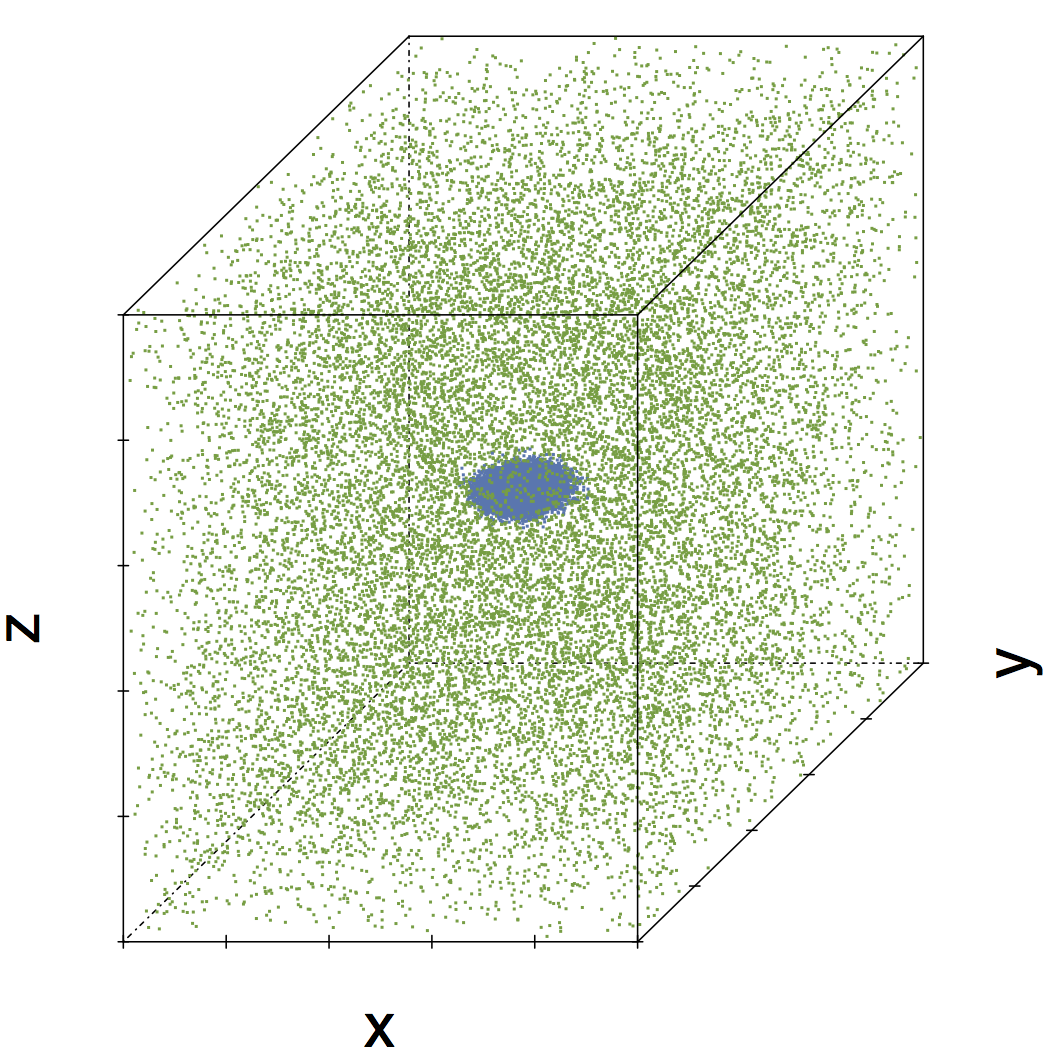
\includegraphics[width=\textwidth]{3/img/datasetplot_baakman_1_60000.png}
	\caption{Set \baakmanOne}
	\label{fig:3:simulated:datasets:baakman1}
\end{subfigure}
% Baakman 2
\begin{subfigure}{0.3\textwidth}
	\centering
	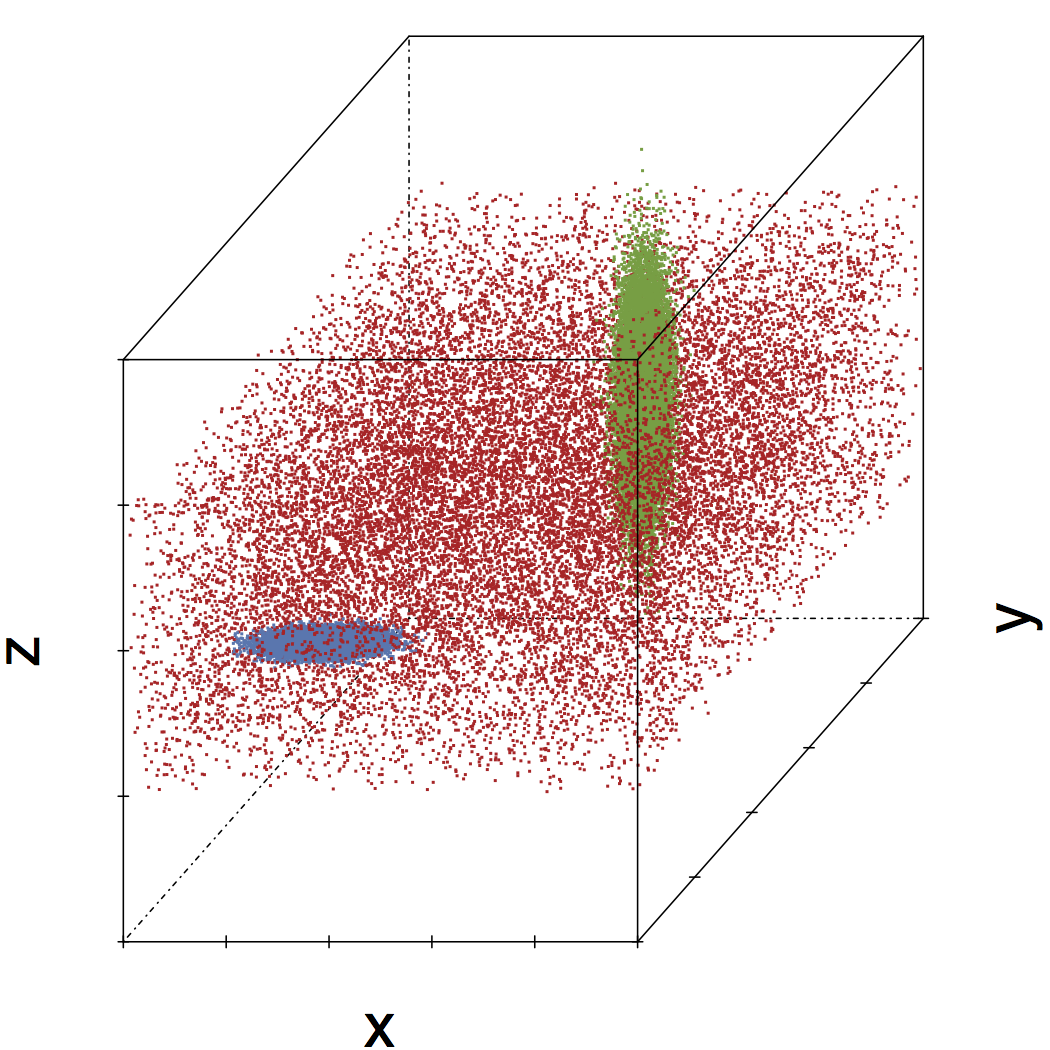
\includegraphics[width=\textwidth]{3/img/datasetplot_baakman_2_60000.png}
	\caption{Set \baakmanTwo}
	\label{fig:3:simulated:datasets:baakman2}
\end{subfigure}	
% Baakman 3
\begin{subfigure}{0.3\textwidth}
	\centering
	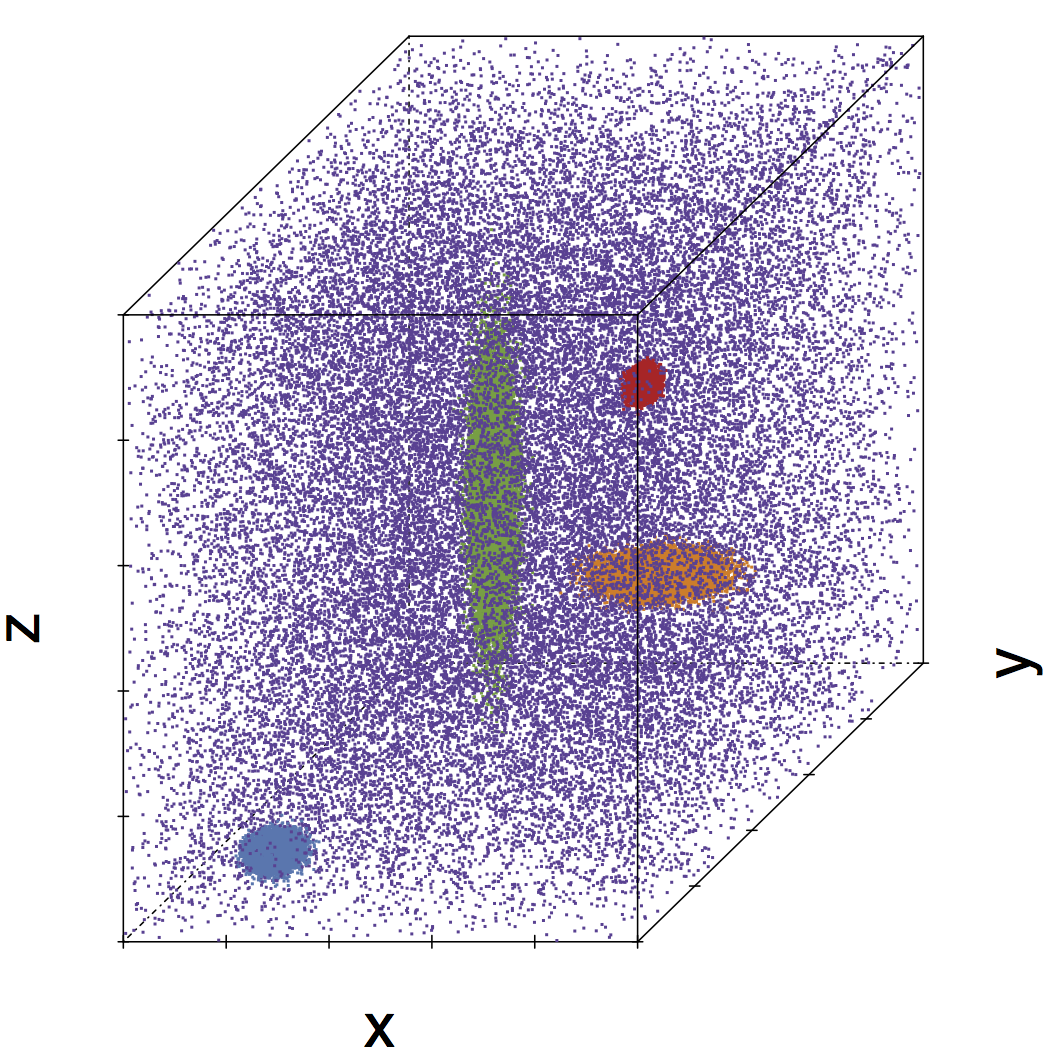
\includegraphics[width=\textwidth]{3/img/datasetplot_baakman_3_120000.png}
	\caption{Set \baakmanThree}
	\label{fig:3:simulated:datasets:baakman3}
\end{subfigure}
% Baakman 4
\begin{subfigure}{0.18\textwidth}
	\centering
	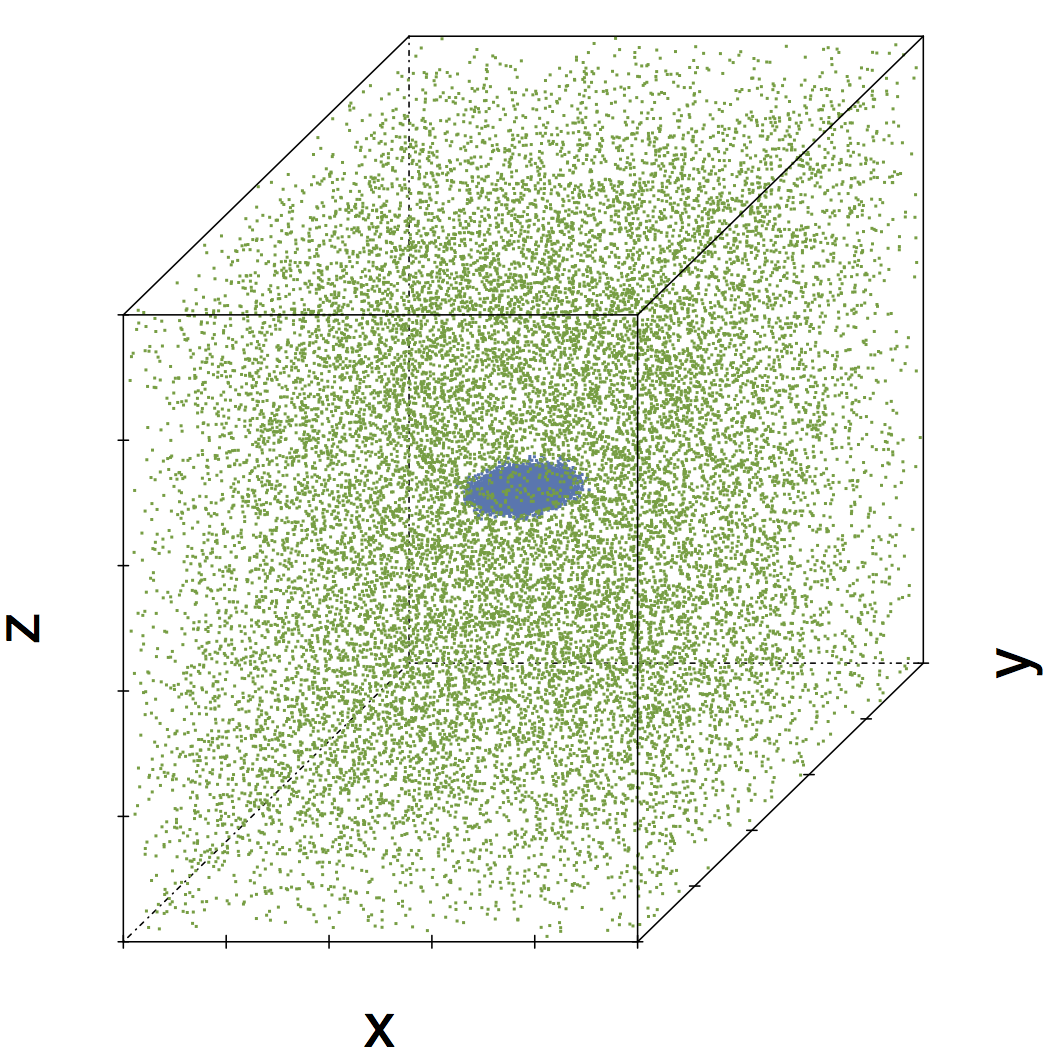
\includegraphics[width=\textwidth]{3/img/datasetplot_baakman_4_60000.png}
	\caption{Set \baakmanFour}
	\label{fig:3:simulated:datasets:baakman4}
\end{subfigure}	
% Baakman 5
\begin{subfigure}{0.18\textwidth}
	\centering
	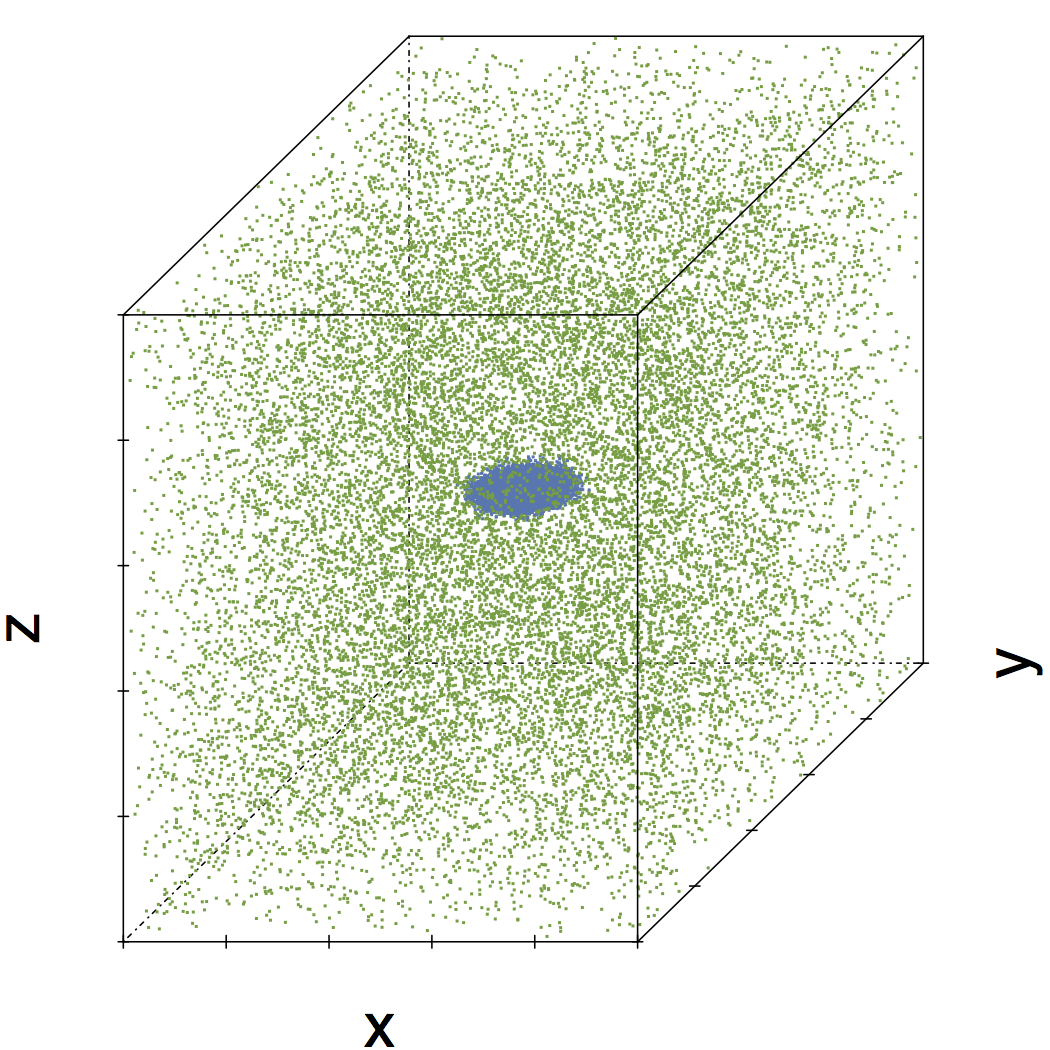
\includegraphics[width=\textwidth]{3/img/datasetplot_baakman_5_60000.png}
	\caption{Set \baakmanFive}
	\label{fig:3:simulated:datasets:baakman5}
\end{subfigure}	